%!TEX root = /Users/simo/Documents/PFC/Chapter2/chapter2.tex
Según se ha establecido mediante el estudio previo, se han diferenciado dos partes muy claras. Incluso así, es posible modularizar el desarrollo de ambas partes en elementos más sencillos, que se irán uniendo con el tiempo.

Simplificando, antes de que la interfaz en Javascript pueda interactuar con el servidor, es necesario que el sistema se haya preparado y sepa como responder a las consultas. Pero para entender totalmente qué tipo de consultas deberá ser capaz de atender, se debe comprender cuál será la implementación de la interfaz, qué elementos básicos se podrán utilizar (líneas, cuadrados, texto, etc.), para así implementar las respuestas adecuadas. Y a la inversa, la interfaz necesita saber cómo serán atendidas sus respuestas para poder tratarlas correctamente.

Es necesario, por tanto, realizar una serialización del trabajo que permita entender qué se necesita de la otra parte, antes de empezar a implementarla. No solamente porque unas partes sean requisito de las otras para que funcionen, sino porque la falta de experiencia con estas dos tecnologías hace que sea necesario un proceso de comprensión previa antes de implementar completamente.

Así pues, los pasos que se han seguido son los siguientes:

\begin{enumerate}
	\item Interfaz Javascript. Implementación de los módulos de renderizado y dibujo.
	\item Sistema. Implementación de los ``modelos'' de las Pizarras y sus Elementos, con	sus controladores y vistas correspondientes, para permitir la introducción, modificación y consulta de nuevas figuras dentro de una Pizarra, y ser consultadas por la interfaz.
	\item Interfaz Javascript. Implementación del módulo de comunicación, que utiliza las vistas implementadas anteriormente de forma adecuada.
	\item Sistema. Extensión del sistema para manejar Usuarios, Grupos y Pizarras. Se añaden las vistas necesarias para que la interfaz pueda realizar consultas sobre los usuarios que participan en una Pizarra.
	\item Interfaz Javascript. Implementación del módulo de usuarios, utilizando las vistas implementadas anteriormente para poder manejar los permisos de los distintos usuarios, así como mantener a los participantes informados de quién está participando.
	\item Proceso de diseño de la web e integrado en el sistema.
	\item Funcionalidades extra: Impresión de documentos.
\end{enumerate}

\section{Javascript: Consideraciones previas}
Debido a las razones explicadas anteriormente, se deduce que Javascript es un lenguaje un tanto peculiar. Su sintaxis en la misma en todos los navegadores, pero no su DOM (Document Object Model), el cual suele cambiar sutilmente de uno a otro. Estas diferencias han hecho que tradicionalmente, saber programar en Javascript signifique conocer en profundidad dichas diferencias, y la forma en que evitarlas.

Los navegadores ``proveen'' a Javascript con dicho DOM, que no es más que una serie de objetos, a modo de librería, con los que poder consultar o modificar cualquier cosa. Por ejemplo, en cualquier momento se puede acceder a los objetos \texttt{navigator, document, window, location, screen}, etc, los cuales contienen una serie de atributos y métodos que se pueden consultar o ejecutar. Por ejemplo, el atributo \texttt{appName} del objeto \texttt{navigator} devuelve una cadena de texto con el identificador del navegador. Así, una forma sencilla de diferenciar los navegadores IE del resto sería mediante una línea como la siguiente:

\begin{verbatim}
if (navigator.appName == "Microsoft Internet Explorer") 
\end{verbatim}

Otro objeto muy importante es el \texttt{document}, a partir del cual se puede acceder y modificar todo el código html. Por ejemplo, mediante la línea siguiente se podría obtener un objeto que representaría la etiqueta \texttt{<svg id=`mainElement`>} :

\begin{verbatim}
var mainElem = document.getElementById("mainElement");
\end{verbatim}

La mayor parte del DOM es similar en todos los navegadores, haciendo las tareas típicas muy simples. Pero es en esas pequeñas diferencias en que Javascript se convierte en algo tedioso y problemático. Con el tiempo Javascript se ha ido popularizando y por lo tanto un mayor número de programadores han dedicado sus esfuerzos al lenguaje, incrementando la cantidad de documentación y librerías disponibles en proporción a dicha popularidad. Era solo cuestión de tiempo que se encontrara una solución a los problemas que se han planteado.

La solución ha aparecido en forma de librerías que permiten hacer las acciones comunes de forma unificada, encargándose ella de distinguir entre navegadores y versiones, y hacer que siempre se ejecuten los comandos apropiados. Existen diferentes librerías para esto, y en este caso se ha decidido usar jQuery. Tomando el ejemplo de querer añadir un evento a un elemento, este es el código típico que se debería ejecutar:

\begin{verbatim}
var elem = document.getElementById("body");
if(naigator.appName == "Microsoft Internet Explorer") {
   elem.attachEvent("onmousedown", doSomething);
} else {
   elem.addEvent("mousedown", false, doSomething);
}
\end{verbatim}

No solo es diferente el nombre de la función para añadir un evento, sino que en IE no se permite definir la política de bubbling, y además los nombres de los eventos son diferentes (onmousedown y mousedown).

El mismo código con jQuery incluida, quedaría así:

\begin{verbatim}
$("body").attach("mousedown",doSomething);
\end{verbatim}

Aunque aparentemente se reduzca el número de líneas, a la hora de ejecutar se tienen que hacer el mismo número de comprobaciones, quedando por tanto en un rendimiento similar, sino peor. Sin embargo, dejando todo este número de comprobaciones ``rutinarias'' de manos de una librería hace que se produzcan menos errores, pues al ser una librería pública usada por un gran número de personas, se puede asumir hayan tenido en cuenta un mayor número de factores de los que uno es capaz trabajando independientemente. Una vez más, debido a una mayor sencillez del código, es posible realizar un trabajo más limpio y libre de errores.

No solo eso, sino que es posible añadir dicha librería directamente de la página de jquery de la siguiente forma:

\begin{verbatim}
<script src="http://jquery.com/jquery-latest.js"></script>
\end{verbatim}

Puesto que un gran número de páginas usan estas librerías hoy en día, la mayoría de la gente ya habrá cargado este archivo anteriormente, reduciendo el tiempo de carga de nuestras páginas para una gran parte de nuestros visitantes, puesto que el código usando jQuery es mucho más reducido, y el cliente ya tendrá en su disco duro dicha librería.

El único problema de estas librerías es que tienen una limitación en cuanto a navegadores soportados. Lamentablemente al estar usando esta librería es posible que se reduzca el número de navegadores soportados por la aplicación, pero se considera que los beneficios de usarla sobrepasan los inconvenientes. Los navegadores soportados son más que razonables, y solamente una persona con un software extremadamente desactualizado tendría algún problema.

\section{Javascript: Renderizado}
Se ha establecido que se utilizará VML para renderizar los elementos en navegadores Internet Explorer, y SVG en el resto, pues es la forma de conseguir llegar al mayor porcentaje de personas de forma que no necesiten instalar nada. Estas son las versiones de los navegadores que soportan dichas tecnologías:

\begin{table}[h]
	\centering
		\begin{tabular}{|c|c|}
			\hline
			Navegador & Versión \\
			\hline
			Internet Explorer & 5.0 \\
			\hline
			Mozilla Firefox & 1.5 \\
			\hline
			Safari & 3.0 \\
			\hline
			Opera & 8.0 \\
			\hline
		\end{tabular}
\end{table}

En principio podría considerarse que cualquier persona con dichos navegadores debería ser capaz de participar en una pizarra, al menos, como espectador, pero estas tecnologías no son las únicas que pueden limitar el rango de navegadores que puedan funcionar. Ya se ha comentado que la librería jQuery tiene unos requerimientos más restrictivos.

\begin{table}[h]
	\centering
		\begin{tabular}{|c|c|}
			\hline
			Navegador & Versión \\
			\hline
			Internet Explorer & 6.0 \\
			\hline
			Mozilla Firefox & 2 \\
			\hline
			Safari & 3.1 \\
			\hline
			Opera & 9.0 \\
			\hline
		\end{tabular}
\end{table}

Es imposible dar un porcentaje exacto de uso de los diferentes navegadores, pues varía dependiendo del grupo de usuarios que tiendan a visitar este tipo de webs, y por tanto, la única forma sería tener estadísticas de dicha web a lo largo de un periodo de tiempo. Sin embargo, tomando el ejemplo de una de las pocas webs que publica sus estadísticas\footnote{\url{http://www.w3schools.com/browsers/browsers_stats.asp}}, los navegadores mencionados comprenden más del 98.5\% del total.

El objetivo de este módulo es que sea capaz de realizar los dibujos de las figuras independientemente del navegador que se esté utilizando. Para ello deberán ejecutarse comandos distintos se esté en Internet Explorer (\texttt{IE} a partir de ahora) o en otro. Se pretende, por lo tanto, proveer una serie de funciones como la siguiente:

\begin{verbatim}
function createLine(here, x1, y1, x2, y2, color, thick, fill)
\end{verbatim}

Dicha función creará una línea que vaya de las coordenadas \texttt{x1,y1} a \texttt{x2,y2}, de color \texttt{color}, con un grueso \texttt{thick}, y con una transparencia del \texttt{fill}\%. Dicho elemento se anidará al elemento padre \texttt{here}.

Los elementos implementados son: línea, polilínea (trazo que pasa por una serie de puntos, como sería el resultado de un trazo a mano alzada), círculo, cuadrado, texto e imagen. Se puede encontrar la especificación de dichas funciones en el anexo, pero son generalmente suficientes para crear, modificar y eliminar satisfactoriamente todos los elementos.

\subsection{Requisitos}
Por desgracia, para que dicho módulo funcione existen una serie de requisitos. Primero, es necesario que el \texttt{HTML} sea el adecuado.

\texttt{VML} necesita dos líneas para que el navegador sepa cómo tiene que representar las directrices.
\begin{verbatim}
<html xmlns="http://www.w3.org/1999/xhtml" 
   xmlns:v="urn:schemas-microsoft-com:vml">

<style>v\:* { behavior: url(#default#VML);}</style>
\end{verbatim}

La primera línea tiene el formato típico de un documento \texttt{XML} formal. Se definen dos espacios de nombres, el princial siendo el de xhtml definido pr el \texttt{W3C}, y el segundo el de la especificación de \texttt{VML} por parte de microsoft, al cual se le añade el prefijo \texttt{v:} . Gracias a esta línea se consigue que se puedan incluir los elementos directamente en el documento, siempre y cuando empiecen por el prefijo \texttt{v:} .

La segunda línea es necesaria para que se puedan aplicar correctamente los estilos a los diferentes elementos. Dicha línea puede añadirse en cualquier punto de la cabecera (entre las etiquetas de \texttt{head}).

En cuanto a \texttt{SVG}, en cualquiera de los navegadores, es necesario que el documento sea de tipo XHTML (el código debe ser XHTML estricto, y que cuando el servidor transmita el documento, el campo \texttt{content-type} debe ser \texttt{application/xhtml+xml}. Para esto basta con cambiar la extensión del archivo a .xhtml, o modificar dicho atributo antes de ser enviado (ruby permite cambiar dicho campo, así como cualquier lenguaje de scripting como podría ser PHP). 

A diferencia de VML, SVG necesita de una etiqueta principal dentro de la cual colgarán los elementos. Debería tener una estructura como la siguiente:

\begin{verbatim}
<svg id="mainElement" xmlns="http://www.w3.org/2000/svg" 
   xmlns:xlink="http://www.w3.org/1999/xlink" 
   preserveAspectRatio="none" height="600px" width="800px">
</svg>
\end{verbatim}

El atributo id permitirá acceder fácilmente a este elemento mediante javascript. Los dos atributos xmlns son también típicos de un documento \texttt{XML}, y añaden las definiciones correspondientes a los elementos \texttt{SVG} y de \texttt{xlink}. Xlink se utiliza para referenciar elementos exteriores al documento, como podrían ser imágenes, y se explicará con más detalle en secciones posteriores. El atributo \texttt{preserveAspectRatio} ayuda a que no se deforme la imagen con posibles redimensionamientos de la ventana, y \texttt{height/width} simplemente indican el tamaño de la imagen SVG (no hay que olvidar, que al fin y al cabo estamos generando una imagen de tipo SVG).

Por último, para todo tipo de navegadores es necesario definir dos variables de Javascript, una que apunte al elemento principal del cual colgarán las etiquetas y otro que apunte al elemento exterior que servirá de referencia a la hora de calcular la posición exacta del ratón respecto al documento. En VML ambos elementos pueden ser el mismo, por lo tanto teniendo un div sería suficiente. Para SVG, sin embargo es necesario que la etiqueta SVG esté contenida dentro de una etiqueta DIV.

La razón por la cual se necesitan dos variables distintas es a causa de las diferencias en cuanto a la estructura proporcionada por el DOM. Objetos \emph{clásicos} del \texttt{HTML} como un DIV traen una serie de funciones y propiedades que el propio navegador proporciona, como son los atributos \texttt{offsetLeft} y \texttt{offsetTop}, los cuales sirven para saber la posición del ratón de forma precisa. La etiqueta SVG, sin embargo, no trae dichos atributos, con lo cual es necesario que esté ubicada dentro de un elemento estructural de HTML.

En el caso de VML esto no es necesario puesto que es posible añadir elementos VML en cualquier parte del código, y solo es necesario tener un DIV para contener todos los elementos bien ordenados y posicionados respecto al marco de lo que sería la pizarra. En SVG, al estar embediendo un documento SVG dentro de un documento XHTML, es necesario que mantenga toda su estructura típica, que es con un elemento base SVG.

\begin{figure}[h!]
\centering
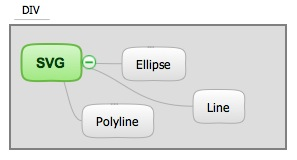
\includegraphics{divsvg.png}
\caption{Esquema del concepto de SVG dentro de un DIV}\label{fig:divsvg}
\end{figure}

Las dos variables a definir son \texttt{mainElem} y \texttt{container}.

\subsection{Implementando}
Todas las funciones de renderizado funcionan de la misma manera. Si se añadiera al código la línea siguiente:
\begin{verbatim}
  <div id="container">
    <v:line from="0,0" to="200,200">
      <v:stroke color="#000000" weight="1" opacity="0.8"/>
    </v:line>
  </div>
\end{verbatim}
se obtendría una línea que iría del punto 0,0 al 200,200 dentro del div contenedor, de color negro (\texttt{\#000000}), de 1 pixel de grosor y una opacidad del 80\%.

Lo que se pretende lograr con el módulo en javascript, es que se pueda ejecutar la línea siguiente:
\begin{verbatim}
  line = new Line(document.getElementById("mainElement"),0,0,200,200,"#000000",1,0.8);
\end{verbatim}
en cualquier momento mediante Javascript, y que automáticamente se cree ese nodo \texttt{<v:line>}. Gracias a que es posible ejecutar código javascript en cualquier evento, es posible crear una línea cuando se pulsa el ratón, e ir modificando sus coordenadas mientras se mueve. No solo eso, sinó que si se recibe alguna información, por ejemplo, mediante Ajax, es posible dibujar dinámicamente elementos a la vez que el servidor los va mandando, sin tener que recargar la página. Es posible usar, por tanto, estas funciones del motor de renderizado tanto para simular el hecho de estar dibujando (motor de dibujo), como para recibir los dibujos que realizan el resto de participantes de una pizarra (módulo de comunicaciones).

Javascript tiene todas las funciones necesarias para modificar el DOM tanto como se desee. Se ha visto que es posible obtener un elemento del código mediante el \texttt{document.getElementById}, y una vez se tiene ese objeto, existen funciones como \texttt{appendChild} para ir modificándolo.

Gracias a jQuery, y a que Javascript es un lenguaje muy relajado sintácticamente, se han podido salvar las distancias entre VML y SVG de forma bastante sencilla. Al final siempre se tiene que implementar cada función dos veces, puesto que la sintaxis de VML y SVG es diferente (hay elementos iguales, pero la sintaxis para crearlos no es la misma), pero estas funciones hacen transparente este proceso. 
